\documentclass{article}
\usepackage{tikz, comment}
\usepackage{pifont}
\usepackage{fontspec, pgfplots}
\usetikzlibrary{arrows, decorations.markings, decorations.pathreplacing}
\begin{comment}
:Title: Not defined yet
:Tags: absolute value rules;properties of equality, equation rules;proper subset;equivalence properties of equality;element of a set
:Prob: 0.7968;0.7932;0.6766;0.6663;0.6076
:Author: Prof.Hu Ji-shan, HKUST
:Slug: No name yet

Description Here.........
\end{comment}
\begin{document}\centering 

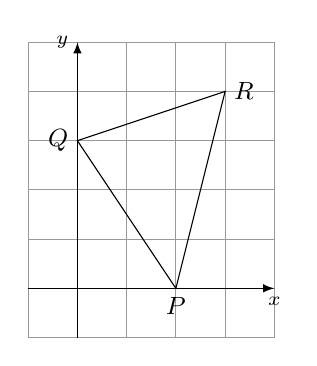
\begin{tikzpicture}[>=latex,xscale=.5*1.25, yscale=.5*1.25][font=\sf\small] 

\draw[xstep=1cm,ystep=1cm,color=gray!80] (-1, -1) grid (4, 5);

\draw[->] (-1, 0) -- (4, 0)node[below] {\scriptsize$x$} ;
\draw[->] (0, -1) -- (0, 5)node[left] {\scriptsize$y$} ;

\draw (2, 0)node[below]{$P$} -- (0, 3)node[left]{$Q$} -- (3, 4)node[right]{$R$} -- cycle;

\end{tikzpicture}
\end{document}